\newpage
% ---- Couverture
% Insert the image as the background for the cover page
\begin{tikzpicture}[overlay,remember picture]
    \node[inner sep=0pt, anchor=south west] at (current page.south west) {
        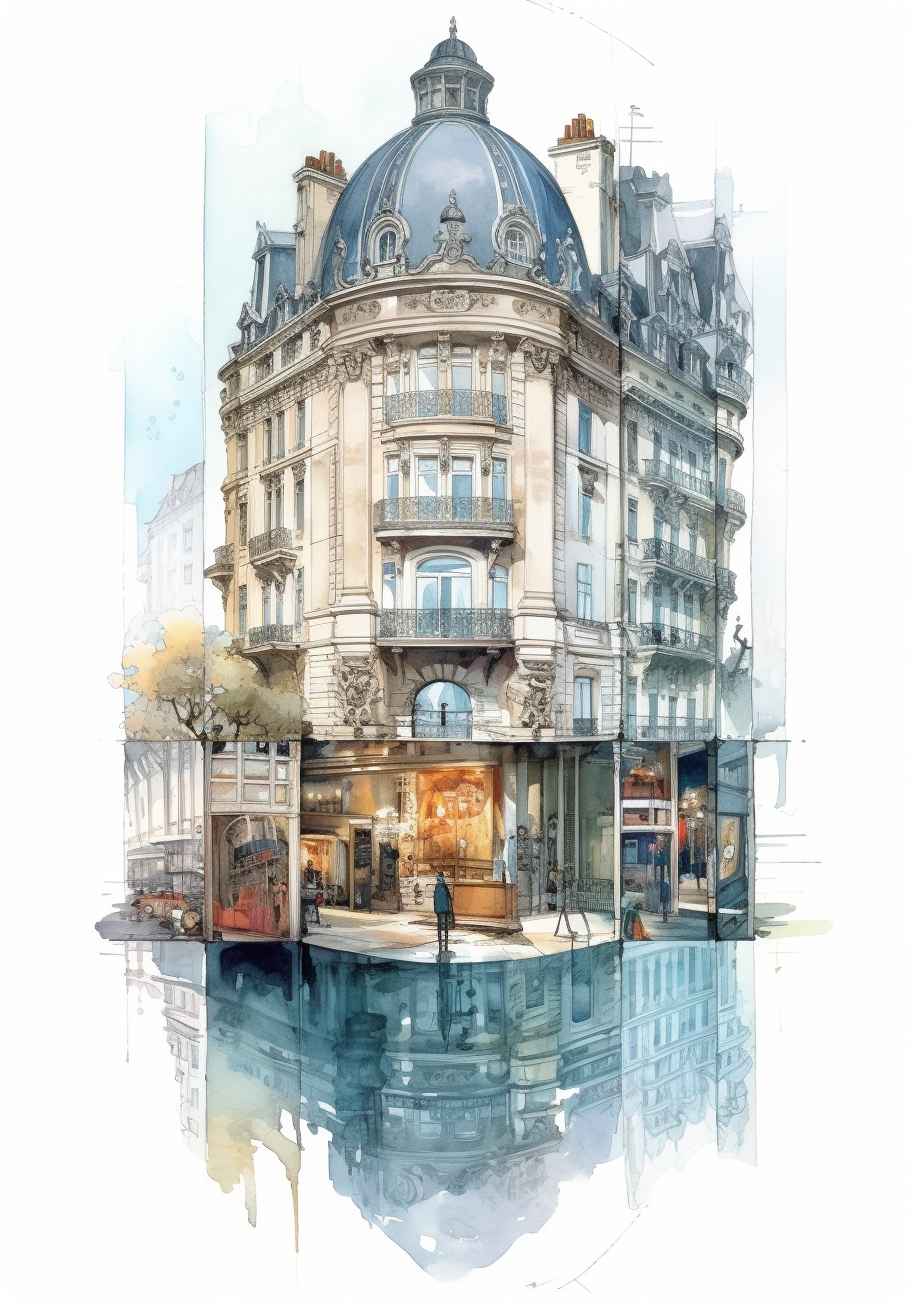
\includegraphics[keepaspectratio, width=\paperwidth]{images/375669df-73f6-4168-9295-19bef29746b5.png}
    };

    % White frame with 0.33 opacity
    \fill[white, opacity=0.33] (current page.south west) rectangle (current page.south east |- current page.center);

    % Title
    \node[align=center] at ($(current page.center)+(0,-5.5)$)
    {
    {\fontsize{45}{72} \fontfamily{cmr}\selectfont \textcolor{black}{\textbf{L'envers du décor}}}\\[0.5cm]
    {\fontsize{30}{72} \fontfamily{cmr}\selectfont \textcolor{black}{\textbf{des Entreprises}}}\\[0.25cm]
    {\fontsize{45}{72} \fontfamily{cmr}\selectfont \textcolor{black}{\textbf{Libérées}}}
    };

    % Author
    \node[align=center] at ($(current page.center)+(0,-10)$)
    {
        {\fontsize{12}{19.2} \textcolor{black}{\selectfont {Kevin Delfour}}}\\[3pt]
    };
\end{tikzpicture}

\newpage
\thispagestyle{empty} % Supprime les en-têtes et pieds de page sur cette page
\mbox{}
% Page blanche

%=========================================
\newpage{}
\thispagestyle {empty}
\begin{titlepage}
    \centering
    \vspace*{3cm}
    {\fontsize{40}{72} \fontfamily{cmr}\selectfont \textcolor{black}{\textbf{L'envers du décor}}}\\[0.5cm]
    {\fontsize{30}{72} \fontfamily{cmr}\selectfont \textcolor{black}{des Entreprises}}\\[0.25cm]
    {\fontsize{40}{72} \fontfamily{cmr}\selectfont \textcolor{black}{Libérées}}\\[2cm]
    {\fontsize{12}{19.2} \textcolor{black}{\selectfont {Kevin Delfour}}}\\[3pt]
    \vfill
\end{titlepage}

%=========================================
\newpage{}
\thispagestyle {empty}
\vspace*{\fill}

\begin{flushleft}

    \textbf{L'envers du décor des Entreprises Libérées}, © Kevin Delfour, 2023 \\[0.25cm]
    \textbf{ISBN : } xxx xxx xxx xx

    \noindent Tous droits réservés. Aucune partie de ce livre ne peut être reproduite, stockée dans un système de recherche documentaire ou transmise sous quelque forme ou par quelque moyen que ce soit, électronique, mécanique, photocopie, enregistrement ou autre, sans l'autorisation préalable écrite de l'auteur ou de l'éditeur, sauf dans le cas de brèves citations intégrées à des critiques ou des articles de presse.

    Toute violation des droits d'auteur est passible de poursuites judiciaires, y compris de réclamations en dommages-intérêts et de demandes d'injonction.

    Certaines images ont été créées en utilisant le service Midjourney par Kévin Delfour, qui détient les droits sur ces images conformément aux termes de service de Midjourney.

\end{flushleft}

%=========================================
\newpage{}
\thispagestyle {empty}

\vspace*{2cm}

\begin{center}
    \vspace*{\fill}
    \parbox{10cm}{
        \begin{center}
            \large{\selectfont
                \textit{"C'est ce que nous faisons aujourd'hui détermine ce que nous serons demain."}
            }

            \vspace{.5cm}\hfill{-- Kevin Delfour}
        \end{center}
    }
    \vspace*{\fill}
\end{center}

%=========================================
\newpage
\thispagestyle{empty} % Supprime les en-têtes et pieds de page sur cette page
\mbox{}
% Page blanche

